\section{approach}
\subsection{Approach Overview}
Our approach takes the coverage data and reported issues as input and outputs the non-covered branches with the associated issues. Figure 1 shows the high level design of Covana. Covana consists of three major components: observer component, pre-processing component and analysis component.
The observer component is implemented as several Pex extensions and is attached to Pex for observing different events and collecting data. It collects the coverage data and reported issues and passed them to the pre-processing component. The pre-processing component remove the useless data and dump the data into binary files. The analysis component consumes the pre-processed data in files, carrys out the analysis on the data and outputs the relevant data for non-covered issues.
\subsection{Observer Component}
The observer component is implemented as three Pex extensions: (1) Branch coverage observer. (2) Field access observer. (3) Issues observer.
\subsubsection{Branch coverage observer}
The branch coverage observer is attached to Pex for collecting the branch coverage data. After all the generated tests are executed, it will enumerate the methods of the class under test, checks the coverage information of each branch inside a method and find out the non-covered branches. As Pex runs on top of MSIL (MicroSoft Intermediate Language) assembly, the observer also collects the IL offset of each non-covered branches for further analysis.
\subsubsection{Field access observer}
Filled in later........ Need to read Nikolai's code
\subsubsection{Issues observer}
The issue observer collects different kinds of issues reported by Pex, such as object creation issues, uninstrumented method issues and testability issues.
\subsection{Pre-processing Component}
The pre-processing component pre-processes the different kinds of data collected by the observer component and filters out the useless data based on some heuristics.
\subsubsection{Filter out useless branch coverage data}
A test suite satisfying all branch coverage criteria always satisfies all statement coverage criteria, but not vice versa. Thus, when we get the data of all the non-covered branches, not all of them are useful for user since we focus on helping user to achieve higher block or statement coverage. 
\begin{figure}
\begin{CodeOut}
\begin{alltt}
    if (x != null) \{
  	   Console.WriteLine("type: " + x.GetType());
    \}
    IEnumerator xe = x.GetEnumerator();
\end{alltt}
\end{CodeOut}
\Caption{Non-covered branch with full block coverage when x is not null}
\label{fig:useless1}
\end{figure}
Figure \ref{fig:useless1} shows an example of code under test which achieves full block coverage but not branch coverage. In the example, x is the class under test and is assumed to be not null. In this case, if x is not null, the test case achieves full block coverage but not full branch coverage since the false branch of ``x != null'' is not covered. However, even we make this branch covered, it won't increase the statement or block coverage as it is already covered. Hence, we could simply filter out such non-covered branches. To find out such kind of non-covered branches, we need to check the coverage of their target statements. If their target statements are already covered, then these non-covered branches are considered useless and could be safely filtered out. (later we may deal with the situation of multi clause, like ``if(x!=null || y != null)'')
\subsubsection{Filter out field access information of covered branches}

\subsection{Analysis Component}

%\begin{figure}%
%\includegraphics[scale=0.4, trim=0 120mm 100mm 0mm]{code1.eps}%l b r t
%\caption{}%
%\label{sample}5t
%\end{figure}

